\documentclass[9pt,conference,a4paper]{IEEEtran}
\IEEEoverridecommandlockouts

\usepackage{graphicx}


\title{Particle Swarm Optimization in Multi-Tensor Imaging}
\author{
	\IEEEauthorblockN{
		Michael Paquette\IEEEauthorrefmark{1},
		Eleftherios Garyfallidis\IEEEauthorrefmark{1},
		Samuel St-Jean\IEEEauthorrefmark{1},
		Pierrick Coup\'e\IEEEauthorrefmark{2},
		Maxime Descoteaux\IEEEauthorrefmark{1}
	}

	\IEEEauthorblockA{\IEEEauthorrefmark{1} Sherbrooke Connectivity Imaging Lab (SCIL), Computer Science Department, Universit\'e de Sherbrooke, Sherbrooke, Canada}
	\IEEEauthorblockA{\IEEEauthorrefmark{2} CNRS Laboratoire Bordelais de Recherche en Informatique (LaBRI), Bordeaux, France}

%	\thanks{This work is supported by your Mom}
}




\begin{document}
\maketitle

For the ISBI HARDI reconstruction challenge 2013, we developed a local estimation method based on Multi-Tensor (MT) fitting with the Particle Swarm Optimization technique (PSO) \cite{kennedy-russell:95}. 
We apply this reconstruction to the DTI and HARDI data categories. 

\bigskip

To fit a MT to the diffusion signal $S = \{S_k\}_{k=0}^M$ with gradient scheme $ \{b_k, g_k\}_{k=0}^M$ is to find some parameters so that $y = \{y_k\}_{k=0}^M$, $y_k = \sum_{i=0}^N f_i e^{-b_k g_k^t D_i g_k}$ resembles the measured signal $S$, where $g_k$ is the k$^{th}$ normalized gradient wavevector and $b_k$ the corresponding b-value, $D_i$ is a rank 2 symmetric tensor with volume fraction $f_i$ and $N$ is the number of compartments in the fit.

\bigskip

To perform the MT fitting, we minimize the fitting error for some cost function, here the squared error between the measured signal and the MT approximation, $ \| S-y \|_2^2 $. 
This minimization is carried on by the particle swarm optimization. The PSO is a stochastic optimization algorithm using population interaction to find the minimum of a function $ f: \mathbf{R}^n \rightarrow \mathbf{R} $. 
It starts by randomly initiating $Np$ particles: points $\Omega^0_j \in \mathbf{R}^n$, and $Np$ velocities: points $v^1_j \in \mathbf{R}^n$. 
These points then evolve into the search space according to $\Omega^{t+1}_j = \Omega^t_j + v^{t+1}_j$ and $ v^{t+1}_j = w v^t_j + \phi_p r_p (p^{t}_j - \Omega^t_j) + \phi_g r_g (g^t - \Omega^t_j)$, where $w$, $\phi_p$ and $\phi_g$ are user tuned parameters, $p^t_j$ is the $j^{th}$ particle's best known position at iteration $t$, $g^t$ is the swarm's best known position at iteration $t$ and $r_p,r_g \sim \mathcal{U}[0,1]$. 
The process is repeated for $Ni$ iterations or until some convergence criterion is met. 
The velocity update formula means that the particles are drawn to the swarm's best known position while being deflected by their own best location and conserving some of their past momentum. 
Particles near $g$ will fully explore that area of the space and find the true local minimum while others will converge there from all over the space, allowing to potentially find new attractor points or finding a better value near their own best known location. 
Finally, the conservation of their previous velocity and its random weighting with $p$ and $g$ allow for the particles to escape non-optimal local minima, potentially attracting to them other particles that are trapped.

\bigskip

For the contest, we compared using the raw DW, the DW denoised with adaptive nonlocal means \cite{manjon-coupe:10} using a rician noise model. 
As proposed in \cite{descoteaux-wiest-daessle-etal:08}, each DW images were processed independently. 

We constrained the MT model to use only prolate tensors and also tested adding an isotropic compartment and fixing the volume fraction to be equal between the non-isotropic compartments.

Since the number of compartments is a meta parameter, we chose as a strategy to overfit at every voxel by always estimating three fiber compartments and to re-estimate with less compartments certain voxels based on two criterion.
We first enforce that no voxel has peaks closer to each other than $\theta^\circ$.
This angular based pruning provides a good cleaning because the peaks tend to converge together when the voxel has been overmodeled.
The only drawback is that we put a hard lower bound on the method's angular resolution.
Secondly, we look at the model complexity of neighboring voxels after the angular pruning to detect outliers. 
A voxel that has more compartments than $\Psi$\% of it's neighborhood is re-estimated with less compartments.

In order to validate which denoising and MT constraints were optimal on the training data, we computed tractography for all the different combinations.
Considering that the given ground truth was a binary connectivity matrices with given ROI, we generated connectivity matrix from track count and used them to qualitatively evaluate each method.
For a specific threshold, we can binarize our matrix and obtain a connectivity error, $\#$ false connections + $\#$ missing connections. A false connection is two regions considered connected for that threshold that are not in the ground truth and a missing connection is two regions not considered connected for that threshold that are in the ground truth.
Looking at that error for different thresholds gives an overview of the validity of the tractogram produced from that method.
Indeed, a good tractogram should allow for a large range of threshold value that gives low connectivity error.

\bigskip

For the final result, for both the DTI dataset (32 directions at b = 1200 s/mm$^2$) and the HARDI dataset (64 directions at b = 3000 s/mm$^2$), we used the denoising from \cite{manjon-coupe:10} for SNR 10 and 20 and no denoising for SNR 30. The MT model fitted had three prolate tensors and one isotropic tensor with fixed equal volume fractions.
The pruning parameters were $\theta = 30^\circ$, $\Psi = 50$\% for DTI and $\theta = 20^\circ$, $\Psi = 50$\% for HARDI.
We submitted the resulting peaks to the contest's organizers. 




\begin{figure}
\centering
\begin{tabular}{c  c}
	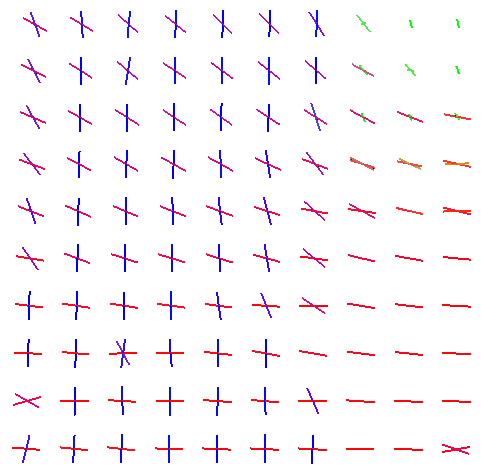
\includegraphics[width=40mm,height=40mm]{dti_slice=22_sel=33_NC=3_iso=1_fr=0_snr=10_type=6_white.png} & 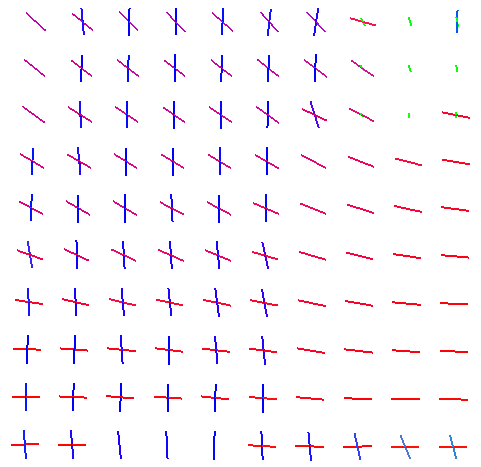
\includegraphics[width=40mm,height=40mm]{hardi_slice=22_sel=33_NC=3_iso=1_fr=0_snr=10_type=6_white.png}\\
\end{tabular}
\caption{Peaks in the testing dataset (ROI = [14:24, 22, 23:33]). Left is DTI, right is HARDI, both result on snr = 10 with denoising from \cite{manjon-coupe:10}.}
\end{figure}



\bibliographystyle{ieeetr}
\bibliography{/media/Data/work/scil-bibtex/scilBibTex.bib}

\
\end{document}


